% Title
\title{Mechanics}
\author{Allan Marbaniang}
\date{Updated : Dec 6 2020}
\maketitle
\tableofcontents

\section{Linearity and non-linearity}
	\begin{frame}
		\begin{itemize}
			\item Suppose there is a function or mapping that does this $f : x \rightarrow y$. Function f takes x and gives y
			
			\item The function is linear if $f(x) = f(x_1) + f(x_2)$. where $x = x_1 + x_2$
			
			\item Suppose we know $f()$ and $y$ but not $x$. Because the function is linear, we can construct solutions $x$ that may be a combination of different solutions $x_i$. The idea is that $f$ should not depend on $x$. It can have other parameters, but not the values of the solution itself. In that case, we would have to find the solution $x$ and also the mapping $f$
			
		\end{itemize}
	
		\begin{block}{Example}
			Take function or map () 
		\end{block}
	\end{frame}




\section{Structural non-linearity introduction}
	\begin{frame}
		\begin{itemize}
			\item What does non-linearity mean ?
			\item What makes a structure non-linear ?
			\item How do you model non-linearity and solve it?
		\end{itemize}
	\end{frame}
	
	\begin{frame}{Structural non-linearity }
		\begin{itemize}
		\item There are different types of non-linearity in a structure 
		\begin{itemize}
			\item Geometrical - $\ve{K(x)x = F }$ where here $\ve{K}$ depends on $\ve{x}$ because $\ve{K}$ changes as you chagne x due to the change in geometry and the large deformation.  
			\item Material - $\ve{K(x)x = F }$ because $\ve{K}$ changes due to the changes in the material property. For eg Youngs modulus may be a function of x. 
		\end{itemize}
		\item $\ve{K}$ is now a function of (x), it means that it can't be solved by using a linear method (Inverting a matrix). 
		\item But the system of equations now has to be linearised about a point. 
		We keep the system of equations as an equality equation $\ve{K(x)x - F} = 0$ . 
		\item We linearise and try to solve the root. At every point we construct the tangent and find a solution, but when we construct the solution at that point, we find the residual and we then use to iterate until convergence. 	
		\end{itemize}
	\end{frame}
		
	\begin{frame}{Problem \#1}
		\begin{figure}
			\centering
			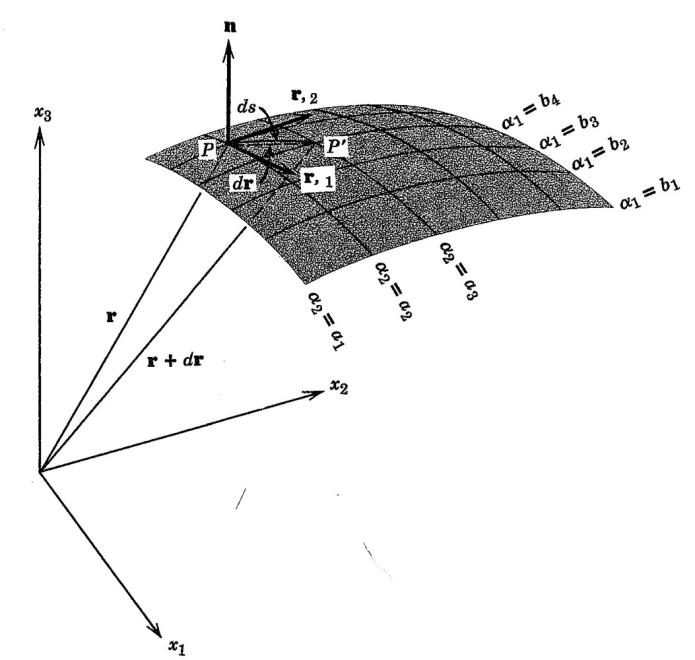
\includegraphics[width=0.7\linewidth]{\pth/continuum/fig1}
			\caption{}
			\label{fig:fig1}
		\end{figure}
		Taking a weightless rigid bar with a torsional spring that resists any moment and a load P at the end. Since the bar is rigid so vertical equilibrium is satisfied at the support without any deformation. However, it can rigidly rotate through the spring.
	\end{frame}
	
	\begin{frame}
		 The moment generated at the end support is	 
		\begin{equation}
			PL cos \theta = M
		\end{equation}
		Taking the equilibrium equation with the spring as $ M = K \theta$ we get
		\begin{align*}
		PL cos \theta = K \theta \\
		\frac{PL}{K} = \frac{\theta}{cos \theta}
		\end{align*}
		\begin{itemize}
			\item If we take $\theta \rightarrow 0$ then $cos \theta \rightarrow 1$
			\item So $P = \dfrac{K}{L}\theta$ which is linear wrt $\theta$
		\end{itemize}
	\end{frame}

	\begin{frame}{Problem \#2}
		\begin{figure}
			\centering
			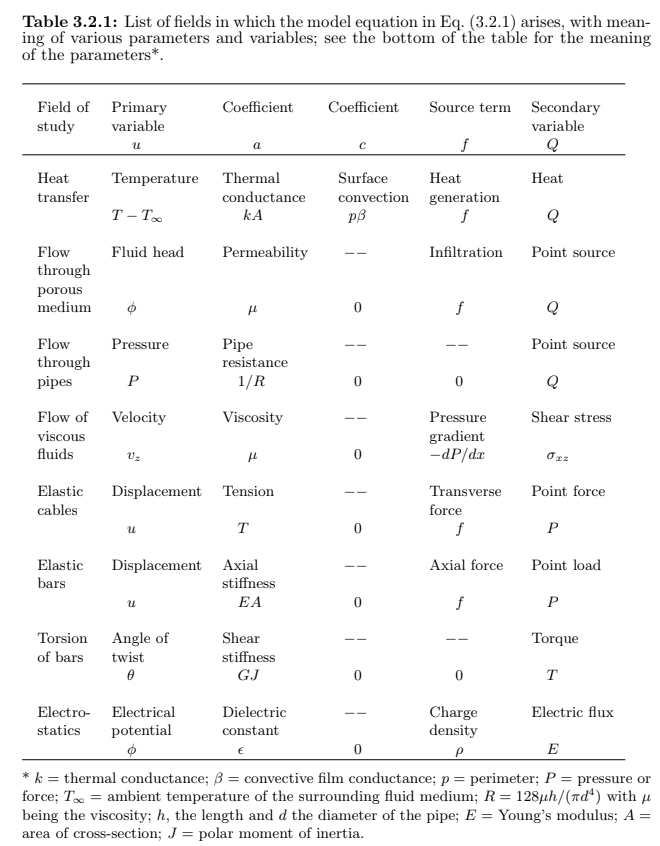
\includegraphics[width=0.4\linewidth]{\pth/continuum/fig2}
			\caption{}
			\label{fig:fig1}
		\end{figure}
		Same problem but now the rigid bar is vertical. This is a very common problem for nonlinearity (I think the previos one is better tho!). Nicely represents buckling of columns
	\end{frame}

	\begin{frame}
		Same equilibrium equation but now the lever arm is different (Because the load along the bar)
		\begin{equation}
		PL sin \theta = M
		\end{equation}
		Taking the equilibrium equation with the spring as $ M = K \theta$ we get
		\begin{align*}
		PL sin \theta = K \theta \\
		\frac{PL}{K} = \frac{\theta}{sin \theta}
		\end{align*}
		\begin{itemize}
			\item If we take $\theta \rightarrow 0$ then $sin \theta \rightarrow 0$ so $M = 0$ (This is one possible equilibrium)
			\item	$\frac{PL}{K} = \frac{\theta}{sin \theta}$ : This is the other
			\item The load $\frac{PL}{K}$ where these two equilibrium equations are possible for the same structure is called the bifurcation point. 
			\item You can imagine that when the load is smaller, it will not buckle and only deform axially so only one equilibrium position ($\theta =0$) is possible. When $\frac{PL}{K}>1$ then the other equilibrium comes to play.
		\end{itemize}
	\end{frame}

	\begin{frame}
		Therefore two solutions  are there :
		\begin{figure}
			\centering
			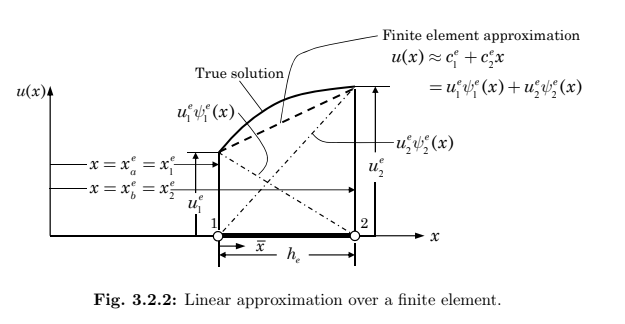
\includegraphics[width=1\linewidth]{\pth/continuum/fig3}
			\label{fig:fig3}
		\end{figure}
		\begin{itemize}
			\item If we linearise our equilibrium equation for small $\theta \rightarrow sin \theta$
			\item We get $(Pl - K)\theta = 0$ and we get our linear eigen value problem with a trivial solution of $\theta = 0$ and a nontrivial solution of $PL = K$. Again we get two equilibrium solutions. $PL = K$ being the buckling load. 
			\item So when we reach that load, it means we have reached the bifurcation point, where multiple equilibrium solutions exist and the rod may buckle dependant on imperfection, lateral load etc. 			
		\end{itemize}
	\end{frame}


\section{Non-Linear strain measures introduction}
	\begin{frame}{Introduction}
		\begin{itemize}
			\item Now suppose of being rigid, the body is deformable that is the relative deformation is introducing strain and stresses
			\item LARGE DISPLACEMENTS + LARGE STRAINS
			\item The first deals with displacements that are large, and therefore while finding the strains, we have to use higher orders of the displacement derivatives
			\item The second deals with ????????????????????????????		
		\end{itemize}
	\end{frame}

	\begin{frame}{One-D strain measures}
		\begin{itemize}
			\item Emphasize its only for One D! But same theory for other dimensions
			\item A strain measure need not be fixed. Sometimes the strain measure we usually use may not be able to model the correct behaviour. When we choose any strain measure, the proper corresponding stress and the  constitutive relationship ($\ve{\sigma = C \varepsilon}$) has to be taken. 
			\item The stress and strain have to be "work compatible". That is they are together used in the strain energy density function. 			
		\end{itemize}
	\end{frame}

	\begin{frame}{One-D strain measures : Types}
		\begin{block}{Engineering strain}
				\begin{itemize}
				\item Engineering strain $\varepsilon_E = \dfrac{l - L}{L} =\dfrac{\Delta }{L}$. l is deformed length, L is initial undeformed
				\item We could have also divided $\Delta$ by l (Change by deformed length). If $l \approx L$ then it would not matter.
				\item $\varepsilon_E $ is the small infinitesimal strain, where the deformed and undeformed lengths are very similar.			
			\end{itemize}
		\end{block}
		\begin{block}{Logarithimic strain}
			\begin{itemize}
			\item The instantaneous strain increment can be thought as $\varepsilon_L = \frac{\Delta_1}{L} + \frac{\Delta_2}{l_1} ...$
			\item Or $d\varepsilon_L = \frac{dl}{l}$  
			\item $\varepsilon_L = \int_{L}^{l}\dfrac{dl}{l} = ln \frac{l}{L}$
			\item The integration is done between two configurations $L \rightarrow l$
			\end{itemize}
		\end{block}	
	\end{frame}

	\begin{frame}{One-D strain measures : Types}
		These strains are more easily extrapolated to continuum (3d cases)
		\begin{block}{Green strain}
			\begin{itemize}
				\item $\varepsilon_G = \dfrac{l^2 - L^2}{2L^2}$ 			
			\end{itemize}
		\end{block}
		\begin{block}{Almansi strain}
			\begin{itemize}
				\item $\varepsilon_A = \dfrac{l^2 - L^2}{2l^2}$ 
			\end{itemize}
		\end{block}	
	
	\begin{itemize}
		\item Suppose $l \approx L$ and therefore $\Delta$ is small
		\item And $l = (L + \Delta)$
		\item $\varepsilon_G = \dfrac{(L + \Delta)^2 - L^2}{2L^2} = \dfrac{(L^2 + \Delta^2 + 2 L \Delta  - L^2)}{2L^2} \approx \dfrac{\Delta }{L}$ (As $\Delta$ is very small and so $\Delta^2$ vanishes)
		
	\end{itemize}
	\end{frame}

	\begin{frame}{Problem \#1}
	\begin{figure}
		\centering
		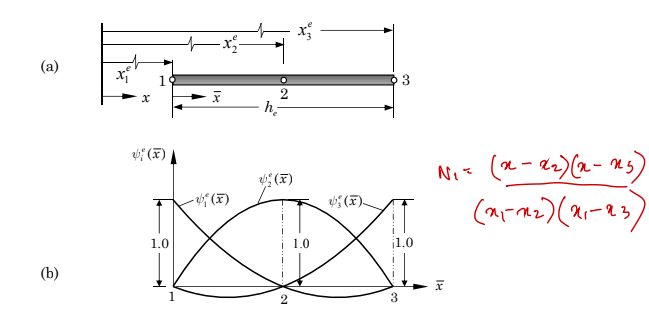
\includegraphics[width=0.6\linewidth]{\pth/continuum/fig4}
		\caption{}
		\label{fig:fig1}
	\end{figure}
	\begin{itemize}
		\item Initial length L, area A, volume V
		\item  Final length l, area a, volume v
		
	\end{itemize}
	\end{frame}

	\begin{frame}
		\begin{itemize}
			\item In defining the equilibrium (Froces = 0 , No moments). We will be defining the internal stress by different strain measures.
			\item Remember that a proper constitutive law has to be taken for a particularly strain measure
			\item Here we have chosen the Cauchy stress and E randomly. The cauchy stress is the actual/true stress in the deformed state. (Or it is the stress in the deformed state which is in equilibrium)
			
		\end{itemize}
		\begin{block}{Using two strain measures}
			Green and logarithmic.
			\begin{itemize}
				\item Cauchy stress (True stress) $\sigma = E \varepsilon$ can be :
				\item $\sigma = E \dfrac{l^2-L^2}{L^2}$
				\item $\sigma = E ln\dfrac{l}{L}$
			\end{itemize}
		\end{block}
	\end{frame}

	\begin{frame}
		\begin{figure}
			\centering
			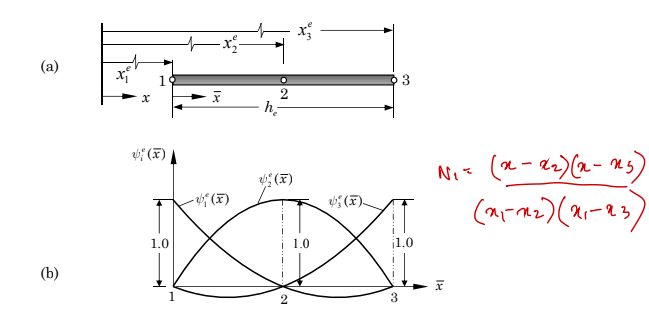
\includegraphics[width=0.3\linewidth]{\pth/continuum/fig4}
			\label{fig:fig1}
		\end{figure}
		\begin{itemize}
		\item The bar will keep moving up until the vertical equilibrium is reached.
		\item Vertical equilibrium at B is $F - T(x)sin \theta(x) = 0$, where $T(x)$ is the internal force and depends on $x$. $\theta$ is also dependant on $x$
		\item Now we can construct a residual function $R(x) =  F - T(x)sin \theta(x)$ where the residual becomes zero for a particular solution of x. \footnote{Note that $\frac{d R}{d x}$ is the tangent stifness $K_{Bx}$ or force in direction B due to displacement x.}  So
		\begin{equation}
		R(x) = \sigma a sin \theta - F = \sigma(x) a \frac{ x}{l} - F
		\end{equation} 	
		\end{itemize}
		
		\begin{block}{Stress dependant on different strain measures}
			\begin{itemize}
				\item $T(x) = E \dfrac{l^2-L^2}{L^2} a \dfrac{x}{l}$  \hfill ($\sigma =  E \varepsilon_G$)
				\item $T(x) = E ln\dfrac{l}{L} a \dfrac{x}{l}$ \hfill	($\sigma =  E \varepsilon_L$)			
			\end{itemize}
		\end{block}
	\end{frame}

	\begin{frame}
		
	\begin{block}{Stress dependant on different strain measures}
		\begin{itemize}
			\item $T(x) = E \dfrac{l^2-L^2}{L^2} a \dfrac{x}{l}$  \hfill ($\sigma =  E \varepsilon_G$)
			\item $T(x) = E ln\dfrac{l}{L} a \dfrac{x}{l}$ \hfill	($\sigma =  E \varepsilon_L$)			
		\end{itemize}
	\end{block}

	\begin{itemize}
		\item l is a function of x, $l^2=D^2+x^2$
		\item R(x) is therefore very nonlinear with respect to x. In R(x), F is not dependant on x. But sometimes it can be the case that the load is also nonlinear.	
	\end{itemize}
	
	\begin{block}{Solving}
		We need to solve the nonlinear equation R(x) = 0
		
		\begin{itemize}
			\item So we use NR, or first order taylor series to linearise R and solve it iteratively
			
			\item $R(x_{i+1}) = R(x_{i}) + \frac{dR}{dx}|_{x_{i}}(x_{i+1}-x{i})$
			\item We want R = 0 , so the value $R(x_{i+1}) = 0$
			\item  $0 = R(x_{i}) + \frac{dR}{dx}|_{x_{i}}(x_{i+1}-x{i})$		
		\end{itemize}
	\end{block}
	\end{frame}

	\begin{frame}
			\begin{figure}
			\centering
			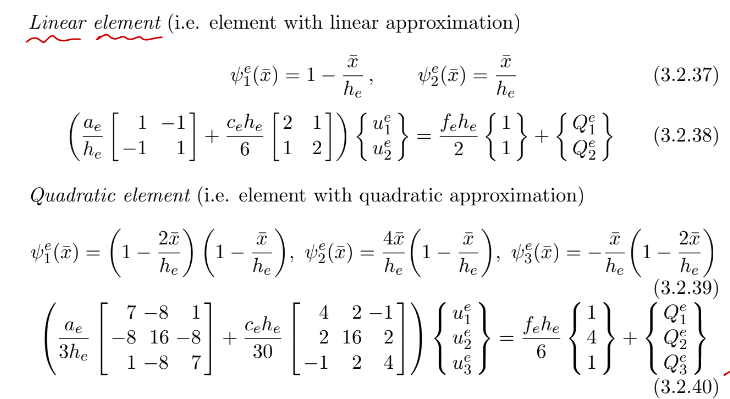
\includegraphics[width=1\linewidth]{\pth/continuum/fig5}
			\label{fig:fig1}
		\end{figure}
	\end{frame}

	\begin{frame}{Summary Problem \#1}
		\begin{itemize}
			\item Regions where x is small, different mesasures gives okay results
			\item We see different behaviour behaviours between the strain measures at higher strain
			\item Snap through behaviour if we increase compressive load too much. Imagine you are pushing the truss down (-x) and suddenly it will roll to the other side. 
			\item If truss  is initially vertical  (Like a column in tension, Therefore no rotation) : Same E should have not been used for both different strain measures. (It seems that the green strain looks good as we expect it to be linear in axial)
			\item Initially horizontal : Stiffening due to tension
			
		\end{itemize}
	\end{frame}

	\begin{frame}{Further insight}
	\begin{itemize}
		\item A comment was made that E should have not been used for the two
	\end{itemize}
	\end{frame}